
\section{Planificación de las Actividades}

Aquí se define el modelo de ciclo de vida de la ontología. El ciclo de vida que se adapta a los escenarios elegidos es el Modelo de Cascada de 6 fases, debido a que serán necesarias las fases de reuso tanto de recursos ontológicos como no-ontológicos, reingeniería, y diseño para la implementación. En la figura \ref{img:secuenciaDeDesarrollo} se muestra el modelo de ciclo de vida a seguir. Se decidió utilizar el Modelo de Ciclo de Vida Cascada ya que el alcance de la ontología es bien delimitado y conocido.

\begin{figure}[h!]
    \centering
    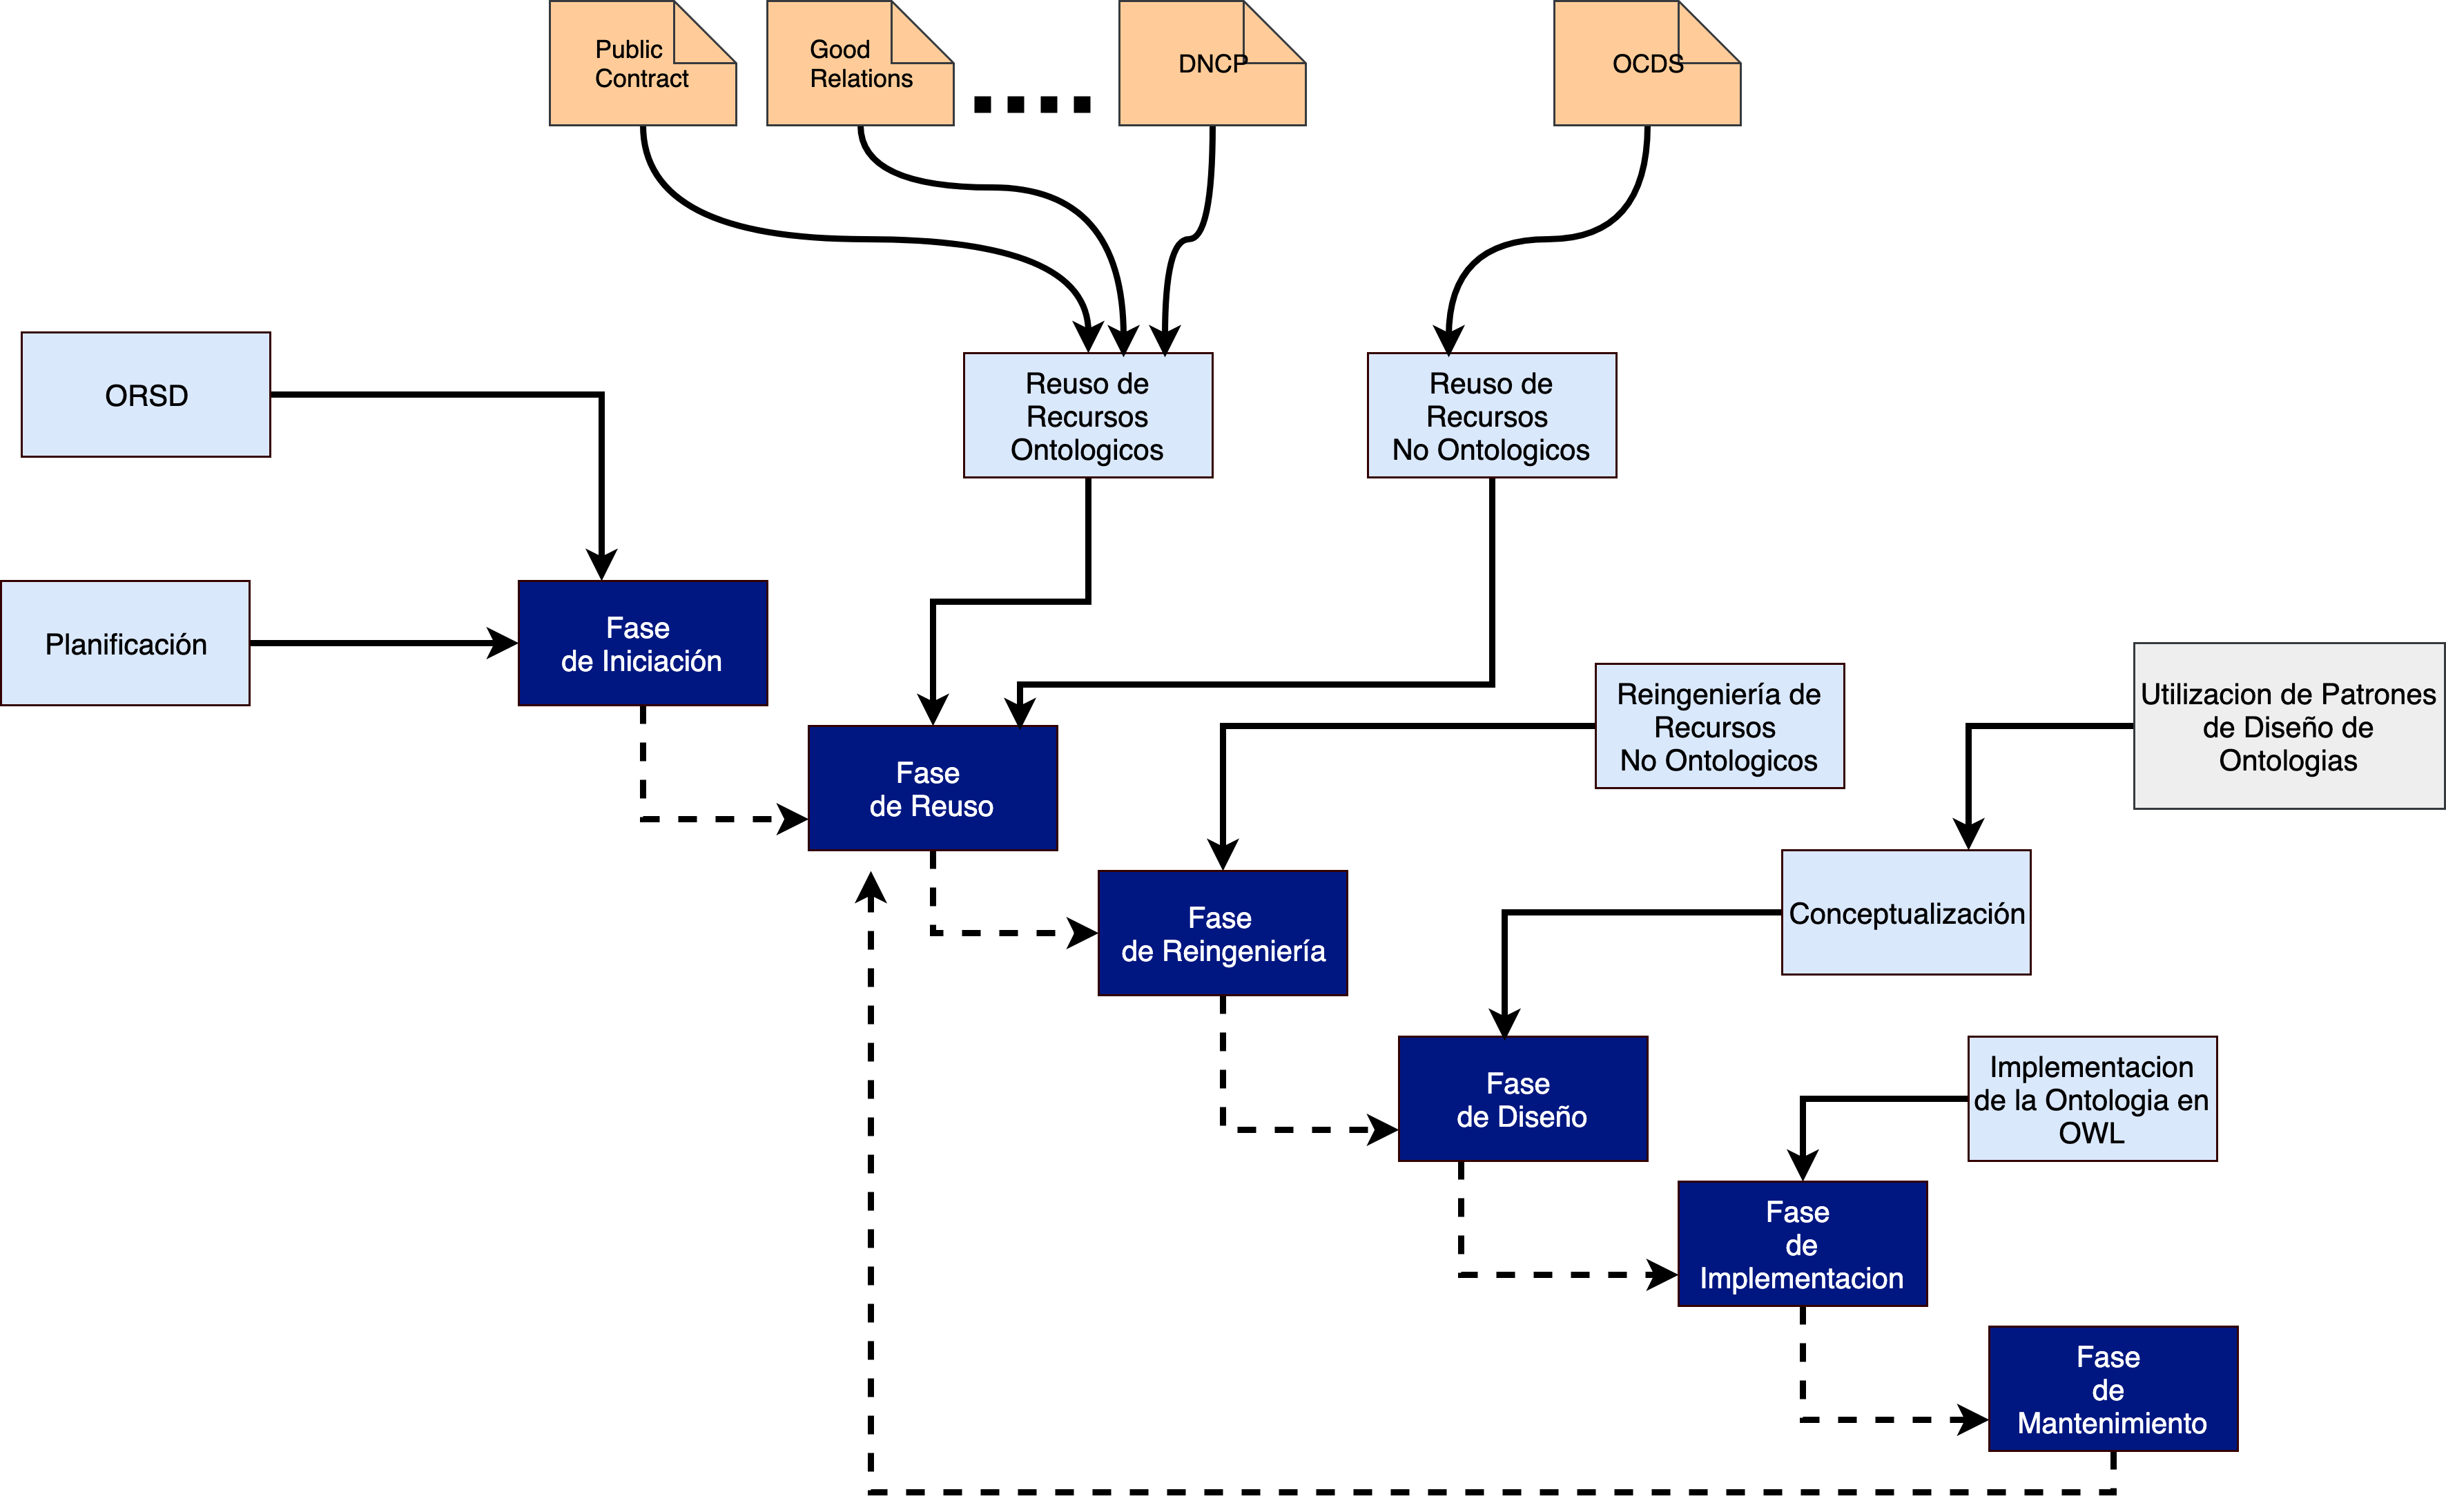
\includegraphics[width=150mm]{figuras/Diagramas-GraficodeSecuenciasDesarrollo.png}
    \caption{Modelo de Ciclo de Vida de desarrollo de la ontología}
    \label{img:secuenciaDeDesarrollo}
\end{figure}

A continuación se citan las actividades divididas en las fases del ciclo de vida a desarrollarse según la metodología NeOn:
\begin{enumerate}
\item Fase 1: Iniciación
\begin{enumerate}
\item Especificación de Requerimientos Ontológicos (ORSD)
\item Planificación 
\end{enumerate}
\item Fase 2: Reuso
\begin{enumerate}
\item Reuso de Recursos No-Ontológicos
\item Reuso de Recursos Ontológicos
\end{enumerate}
\item Fase 3: Reingeniería
\begin{enumerate}
\item Reingeniería de Recursos No-Ontológicos
\end{enumerate}
\item Fase 4: Diseño
\begin{enumerate}
\item Conceptualización de la Ontología
\end{enumerate}
\item Fase 5: Implementación
\item Fase 6: Mantenimiento

\end{enumerate}

Una vez terminada la planificación se procede al desarrollo de cada una de las demás actividades siguiendo el orden de las fases. La explicación de cada una de las actividades se describen a continuación en este documento.
